%%%%%%%%%%%%%%%%%%%%%%%%%%%%%%%%%%%%%%%%%%%%%%%%%%%%%%%%%%%%%%%%%%%%%%%%%%%%%%%%%%%%%%%%%%%%%%%%%%%
%%%%%%%%%%%%%%%%%%%%%%%%%%%%%%%%%%%%%%%%%%%%%%%%%%%%%%%%%%%%%%%%%%%%%%%%%%%%%%%%%%%%%%%%%%%%%%%%%%%
%%%%%%%%%%%%%%%%%%%%%%%%%%%%%%%%%%%%%%%%%%%%%%%%%%%%%%%%%%%%%%%%%%%%%%%%%%%%%%%%%%%%%%%%%%%%%%%%%%%
\documentclass[12pt,dvipdfmx]{beamer}
%%%%%%%%%%%%%%%%%%%%%%%%%%%%%%%%%%%%%%%%%%%%%%%%%%%%%%%%%%%%%%%%%%%%%%%%%%%%%%%%%%%%%%%%%%%%%%%%%%%%%%
% pdfの栞・プロパティの字化けを防ぐ
\usepackage{atbegshi}
%\AtBeginShipoutFirst{\special{pdf:tounicode 90ms-RKSJ-UCS2}} %Windows
\AtBeginShipoutFirst{\special{pdf:tounicode EUC-UCS2}} %Linux, Mac
\usepackage{hyperref}
%%%%%%%%%%%%%%%%%%%%%%%%%%%%%%%%%%%%%%%%%%%%%%%%%%%%%%%%%%%%%%%%%%%%%%%%%%%%%%%%%%%%%%%%%%%%%%%%%%%%%%
%%%
%%% テーマの指定、省略時は default になる
%%%

 % フレームの指定、省略可
%%%%%%%%%%%%%%%%%%%%%%%%%%%% THEME
  %\usetheme{AnnArbor}
  %\usetheme{Antibes}
  %\usetheme{Bergen}
  %\usetheme{Berkeley}
  %\usetheme{Berlin}
  \usetheme{Boadilla}
  %\usetheme{boxes}
  %\usetheme{CambridgeUS}
  %\usetheme{Copenhagen}
  %\usetheme{Darmstadt}
  %\usetheme{default}
  %\usetheme{Dresden}
  %\usetheme{Frankfurt}
  %\usetheme{Goettingen}
  %\usetheme{Hannover}
  %\usetheme{Ilmenau}
  %\usetheme{JuanLesPins}
  %\usetheme{Luebeck}
  %\usetheme{Madrid}
  %\usetheme{Malmoe}
  %\usetheme{Marburg}
  %\usetheme{Montpellier}
  %\usetheme{PaloAlto}
  %\usetheme{Pittsburgh}
  %\usetheme{Rochester}
  %\usetheme{Singapore}
  %\usetheme{Szeged}
  %\usetheme{Warsaw}

% 省略可
%%%%%%%%%%%%%%%%%%%%%%%%%%%% COLOR THEME
  %\usecolortheme{albatross}
  %\usecolortheme{beetle}
  %\usecolortheme{crane}
  %\usecolortheme{default}
  %\usecolortheme{dolphin}
  %\usecolortheme{dove}
  %\usecolortheme{fly}
  %\usecolortheme{lily}
  %\usecolortheme{orchid}
  %\usecolortheme{rose}
  %\usecolortheme{seagull}
  %\usecolortheme{seahorse}
  %\usecolortheme{sidebartab}
  %\usecolortheme{structure}
  %\usecolortheme{whale}

% ヘッダ、フッタ、フレーム等を指定、省略可
  %%%%%%%%%%%%%%%%%%%%%%%%%%%% OUTER THEME
  %\useoutertheme{default}
  %\useoutertheme{infolines}
  %\useoutertheme{miniframes}
  %\useoutertheme{shadow}
  %\useoutertheme{sidebar}
  %\useoutertheme{smoothbars}
  %\useoutertheme{smoothtree}
  %\useoutertheme{split}
  %\useoutertheme{tree}

% タイトル、section, itemize/enumerate 環境、
% theorem 環境、図, 参考文献などのスタイルを指定、
% 省略可
  %%%%%%%%%%%%%%%%%%%%%%%%%%%% INNER THEME
  %\useinnertheme{circles}
  %\useinnertheme{default}
  %\useinnertheme{inmargin}
  \useinnertheme{rectangles}
  %\useinnertheme{rounded}


%\usefonttheme{}	% 省略可
%\logo{}		% 省略可

%%%%%%%%%%%%%%%%%%%%%%%%%%%%%%%%%%%%%%%%%%%%%%%%%%%%%%%%%%%%%%%%%%%%%%%%%%%%%%%%%%%%%%%%%%%%%%%%%%%
%%%%%%%%%%%%%%%%%%%%%%%%%%%%%%%%%%%%%%%%%%%%%%%%%%%%%%%%%%%%%%%%%%%%%%%%%%%%%%%%%%%%%%%%%%%%%%%%%%%
%%%%%%%%%%%%%%%%%%%%%%%%%%%%%%%%%%%%%%%%%%%%%%%%%%%%%%%%%%%%%%%%%%%%%%%%%%%%%%%%%%%%%%%%%%%%%%%%%%%
% navi. symbolsは目立たないが,dvipdfmxを使うと機能しないので非表示に
\setbeamertemplate{navigation symbols}{}

% 各種パッケージ
\usepackage{graphicx}
%\usepackage{url,cite}
\usepackage{amsmath}
\usepackage{amsthm} \theoremstyle{definition} %theorem環境が斜体になるので注意
\usepackage{amssymb} % AMS-TeX
\usepackage{setspace}

% \AtBeginSection[] % Do nothing for \section*
% { \begin{frame}<beamer> \frametitle{}
%    \tableofcontents[currentsection,subsectionstyle=hide]
%  \end{frame} } 

%appendixをページカウントしない
\newcommand{\backupbegin}{
   \newcounter{framenumberappendix}
   \setcounter{framenumberappendix}{\value{framenumber}}
}
\newcommand{\backupend}{
   \addtocounter{framenumberappendix}{-\value{framenumber}}
   \addtocounter{framenumber}{\value{framenumberappendix}} 
}

%%%%%%%%%%%%%%%%%%%%%%%%%%%%%%%%%%%%%%%%%%%%%%%%%%%%%%%%%%%%%%%%%%%%%%%%%%%%%%%%%%%%%%%%%%%%%%%%%%%%%%
% 本文・数式フォント
%\usepackage{palatino,mathpazo}
%\usepackage{times,mathptmx}
\usepackage[varg]{txfonts}
%\usepackage[varg]{pxfonts}

% \mathcal(\cal)の扱い
%\DeclareMathAlphabet{\mathcal}{OMS}{cmsy}{m}{n} %computer modern
%\DeclareMathAlphabet{\mathcal}{OMS}{txsy}{m}{n} %txfont
%\usepackage[psamsfonts]{eucal} % euler

% mathptmx時に数式モードのvをtxfontから借りる
% \DeclareSymbolFont{lettersA}{U}{txmia}{m}{it}
% \SetSymbolFont{lettersA}{bold}{U}{txmia}{bx}{it}
% \DeclareFontSubstitution{U}{txmia}{m}{it}
% \DeclareMathSymbol{v}{\mathalpha}{lettersA}{"33} %"


%上線 widebar, Widebar
\usepackage{accents}
\makeatletter
\def\widebar{\accentset{{\cc@style\underline{\mskip11mu}}}}
\makeatother


%%%%%%%%%%%%%%%%%%%%%%%%%%%%%%%%%%%%%%%%%%%%%%%%%%%%%%%%%%%%%%%%%%%%%%%%%%%%%%%%%%%%%%%%%%%%%%%%%%%%%%

% 定理環境
% \newtheorem{theorem}{Theorem}
% \newtheorem{lemma}[theorem]{Lemma}
% \newtheorem{corollary}[theorem]{Corollary}
% \newtheorem{definition}[theorem]{Definition}
% \newtheorem{example}[theorem]{Example}
\newtheorem{proposition}{Proposition}
\newtheorem{remark}{Remark}

%%%%%%%%%%%%%%%%%%%%%%%%%%%%%%%%%%%%%%%%%%%%%%%%%%%%%%%%%%%%%%%%%%%%%%%%%%%%%%%%%%%%%%%%%%%%%%%%%%%%%%
% 各種コマンド定義等
\def\Fig#1{Fig.\@\ref{#1}}
\def\Table#1{Table~\ref{#1}}
\def\Eq#1{Eq.\@(\ref{#1})}
\def\Eqs#1{Eqs.\@(\ref{#1})}
\def\Thm#1{Theorem~\ref{#1}}
\def\Lma#1{Lemma~\ref{#1}}
\def\Sect#1{Section~\ref{#1}}
\def\Rmk#1{Remark~\ref{#1}}
\def\Prop#1{Proposition~\ref{#1}}
\def\Coro#1{Corollary~\ref{#1}}
\def\Def#1{Definition~\@\ref{#1}}
\def\Prob#1{Problem~\@\ref{#1}}
\def\ie{{i.\@e.\@,~}}
\def\eg{{e.\@g.\@,~}}
\def\etal{{et al.}}

% 数式環境用
\def\rank{\mathsf{rank}\, }
\def\dim{\mathsf{dim}\, }
\def\rspace{\mathsf{span}}
\def\supp{\mathsf{supp}}
%\def\vec#1{\mathbf{#1}}
\def\F{\mathbb{F}}
\def\wt{\mathsf{wt}}
\def\c{\mathcal{C}}
\def\dc{\mathcal{C}^{\perp}}
\def\d{\mathcal{D}}
\def\dd{\mathcal{D}^{\perp}}
\def\g{\mathcal{G}}
\def\dg{\mathcal{G}^{\perp}}
\def\p{\mathcal{P}}
% \def\rspace{\mathsf{span}}
\def\supp{\mathsf{supp}}
\def\ker{\mathsf{Ker\ }}

%\def\bari#1{\{\widebar{#1}\}}
\def\bari#1{\,\overline{{\!\{#1\}\!}}\,}
%\def\bari#1{\bar{\{#1\}}}
\def\vecxi{Z_{\bari{i}}}
%\def\vecsxi{\vec{z}_i}
\def\tvector{X}
\def\tpackets{X_1,\dots,X_n}
\def\mvector{S}
\def\mpackets{S_1,\dots,S_l}
\def\rvector{Y}
\def\wvector{W}
\def\cvector{C}
\def\cword{C_{1},\dots,C_{l+n}}
\def\pcword{C_{l+1},\dots,C_{l+n}}
\def\randvector{R}

\def\compmat{\Phi}

%%%%%%%%%%%%%%%%%%%%%%%%%%%%%%%%%%%%%%%%%%%%%%%%%%%%%%%%%%%%%%%%%%%%%%%%%%%%%%%%%%%%%%%%%%%%%%%%%%%
%%%%%%%%%%%%%%%%%%%%%%%%%%%%%%%%%%%%%%%%%%%%%%%%%%%%%%%%%%%%%%%%%%%%%%%%%%%%%%%%%%%%%%%%%%%%%%%%%%%
%%%%%%%%%%%%%%%%%%%%%%%%%%%%%%%%%%%%%%%%%%%%%%%%%%%%%%%%%%%%%%%%%%%%%%%%%%%%%%%%%%%%%%%%%%%%%%%%%%%
%%%
%%%  日本語フォントをゴシックに、数式フォントを太字に変更する
%%%
\renewcommand{\kanjifamilydefault}{\gtdefault}
\renewcommand{\familydefault}{\sfdefault}

\setbeamerfont{title}{size=\large,series=\bfseries}
\setbeamerfont{frametitle}{size=\large,series=\bfseries}
%\setbeamertemplate{frametitle}[default][center]
\usefonttheme{professionalfonts} 

%\mathversion{bold} %数式フォントを太字に

%\def\vec#1{\mbox{\boldmath $#1$}}


%\logo{\includegraphics[width=2cm]{titech_logo.eps}}

%\setbeamertemplate{caption}[numbered]
%%%
%%% 著者など
%%%
\title[E2E Security with JS 04]{JavaScriptによるEnd-to-Endセキュリティ}
\subtitle{第4回 データの真正性・本人確認のためのテクニック 編}
\author[Jun Kurihara]{栗原 淳}
\institute[]{}
\date[Oct. 3x, 2019]{2019年10月3x日}

%%%%%%%%%%%%%%%%%%%%%%%%%%%%%%%%%%%%%%%%%%%%%%%%%%%%%%%%%%%%%%%%%%%%%%%%%%%%%%%%%%%%%%%%%%%%%%%%%%%
%%%%%%%%%%%%%%%%%%%%%%%%%%%%%%%%%%%%%%%%%%%%%%%%%%%%%%%%%%%%%%%%%%%%%%%%%%%%%%%%%%%%%%%%%%%%%%%%%%%
%%%%%%%%%%%%%%%%%%%%%%%%%%%%%%%%%%%%%%%%%%%%%%%%%%%%%%%%%%%%%%%%%%%%%%%%%%%%%%%%%%%%%%%%%%%%%%%%%%%
%%%%%%%%%%%%%%%%%%%%%%%%%%%%%%%%%%%%%%%%%%%%%%%%%%%%%%%%%%%%%%%%%%%%%%%%%%%%%%%%%%%%%%%%%%%%%%%%%%%
%%%%%%%%%%%%%%%%%%%%%%%%%%%%%%%%%%%%%%%%%%%%%%%%%%%%%%%%%%%%%%%%%%%%%%%%%%%%%%%%%%%%%%%%%%%%%%%%%%%

\begin{document}

\begin{frame}
\titlepage
\end{frame}

%%%%%%%%%%%%%%%%%%%%%%%%%%%%%%%%%%%%%%%%%%%%%%%%%%%%%%%%%%%%%%%%%%%%%%%%%%%%%%%%%%%%%%%%%%%%%%%%%%%
\section{はじめに}
\begin{frame}
 \centering
 {\Large はじめに}
\end{frame}

\begin{frame}
\frametitle{はじめに}
第1,2,3回では
\begin{itemize}
 \item End-to-End (E2E) セキュリティの原則と必要性
 \item JavaScriptでAESを正しく・安全に暗号化する方法
 \item JavaScriptでRSA暗号・楕円曲線暗号を使ってを正しく・安全に暗号化する方法
\end{itemize}
を勉強した。


\vspace{2ex}

今回は、第3回で懸案事項だった「データのやり取りしてる相手って本当に正しい相手?」を保証する方法を学んでいく。
\end{frame}
\begin{frame}
 
\end{frame}

\begin{frame}

\begin{block}{\small この講義で最終的に学びたいこと}
\begin{itemize}
\item 
\end{itemize}
\end{block}

細かい話もするが、数式は使わない。

「イメージ」と「コードの流れ&その流れの必要性」をつかめるようにする。
\end{frame}

\begin{frame}
\frametitle{発表者紹介}
{\Large 栗原 淳 (Jun Kurihara)}
\begin{itemize}
 \item (株)ゼタント 主任研究員\\
(株) 国際電気通信基礎技術研究所(ATR) 連携研究員
 \item 博士(工学), \\
 専門: セキュリティ、応用数学、システムアーキテクチャとか
 \item  Webシステム(フロントエンド・バックエンド)を作ったり、論文他のアルゴリズムを実装したり、研究して論文書いたり、セキュリティ技術中心に手広くやってます。
 \item GitHub: \url{https://github.com/junkurihara}\\
LinkedIn: \url{https://www.linkedin.com/in/junkurihara}
\end{itemize}
\end{frame}

\begin{frame}
\frametitle{この講義の対象と事前準備}
対象:
\begin{itemize}
\item 暗号・セキュリティ技術に興味がある初学者
\item Webに暗号技術を導入したいWeb系のエンジニア
\end{itemize}

\vspace{2ex}

必須ではないが触って楽しむのには必要な事前準備:
\begin{itemize}
\item Bash, Gitが使えるようになっていること
\item Node.js, npm, yarnが使えるようになっていること
\item Google Chrome系ブラウザ and/or Firefoxが利用可能なこと
\end{itemize}
\end{frame}

\begin{frame}
今後の予定(暫定)
\begin{enumerate}
 \item \textcolor{gray}{導入\&JSの暗号化コードを触ってみる}
 \item \textcolor{gray}{AESを正しく・安全に暗号化するには?}
 \item \textcolor{gray}{公開鍵暗号はどうやって使う?その使い方のコツは?}
 \item \alert{ハッシュ・MAC・署名、それぞれの使い所と使い方は?} ← 今日はココ
 \item \textcolor{gray}{RFCにまつわるあれこれ(証明書・鍵フォーマット・etc...)}
\end{enumerate}
「こういうのを知りたい」というリクエストがあれば是非。

マニアックすぎて最後のRFCの話題はやるかどうか不明…

\vspace{2ex}

\underline{セカンドシーズンも検討中。}\footnote[frame]{場所等変えてもっと来やすい場所へ。。。}
\end{frame}



%%%%%%%%%%%%%%%%%%%%%%%%%%%%%%%%%%%%%%%%%%%%%%%%%%%%%%%%%%%%%%%%%%%%%%%%%%%%%%%%%%%%%%%%%%%%%%%%%%%
\section{まとめ}
\begin{frame}
 \centering
 {\Large まとめ}
\end{frame}

\begin{frame}
\frametitle{まとめ}
お疲れ様でした。

\begin{itemize}
\item 
\end{itemize}
\end{frame}


\begin{frame}
\frametitle{次回は}
% \begin{itemize}
%  \item 内容: 
% \begin{itemize}
%  \item 暗号化に加えて、MAC・署名を使ってみよう(数学的なことはやらない)
%  \item まずはハッシュ: SHA2, SHA3
%  \item 共通鍵ベース: HMAC/CMAC
%  \item 公開鍵ベース: RSA Signature/ECDSA
% \end{itemize}
%  \item 日時: 2019年10月31(?)日(木曜日) 19:00- (2週間後)
%  \item 場所: ブロックチェーンハブ (ここ)
%  \item 発表者: (また) 栗原
% \end{itemize}
\end{frame}


\begin{frame}
\frametitle{宣伝: iTransfy by Zettant}
\begin{center}
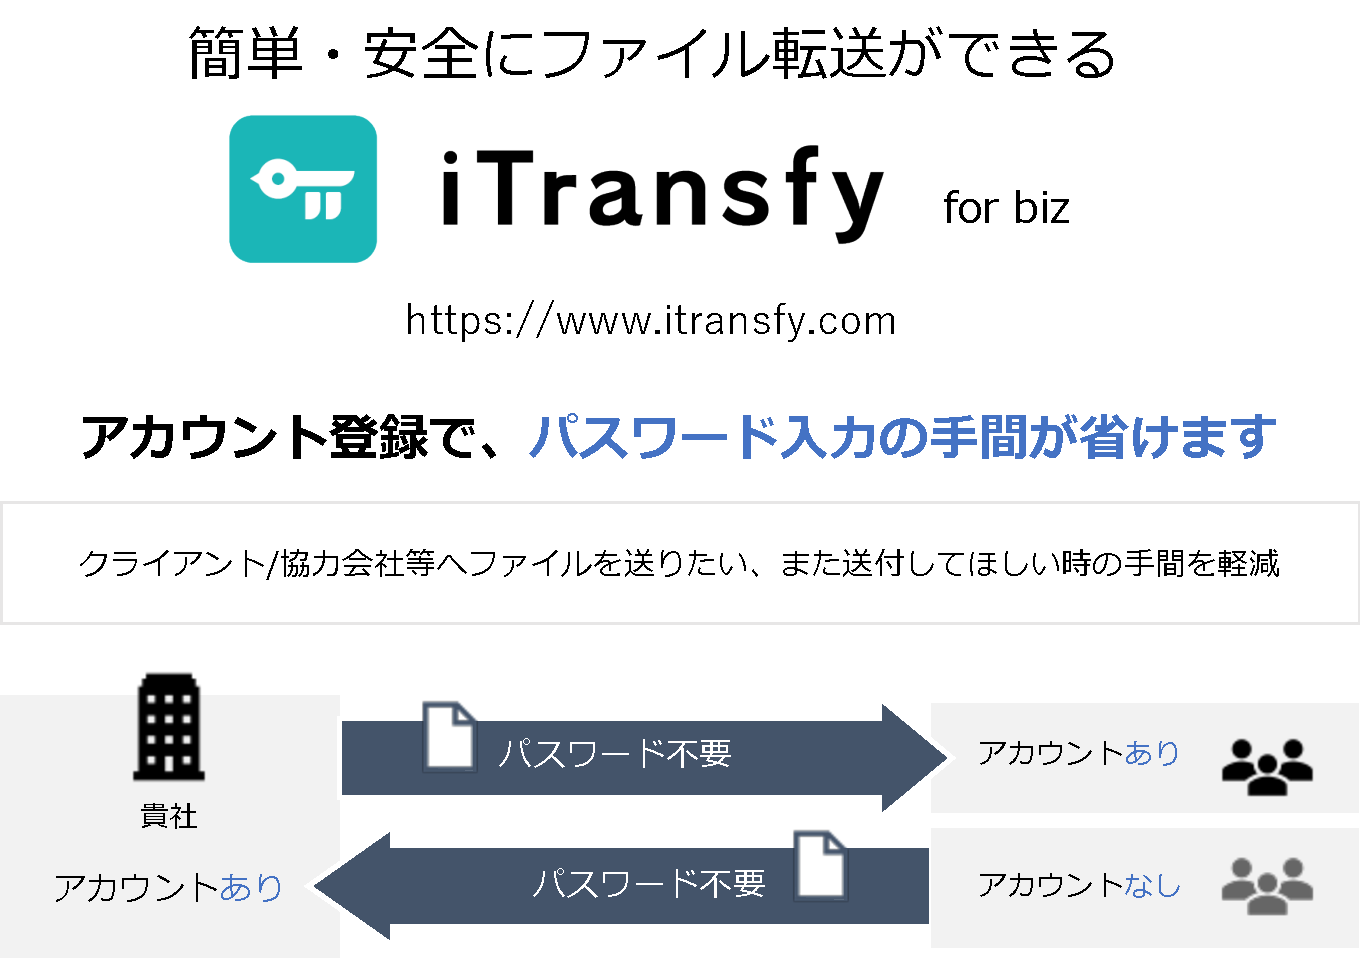
\includegraphics[width=0.9\linewidth]{FigsZettant/itransfy.pdf} 
\end{center}
\end{frame}

\begin{frame}
\frametitle{宣伝: 株式会社ゼタント}
\begin{tabular}{cc}
\begin{minipage}[b]{0.3\linewidth}

\includegraphics[width=\linewidth]{FigsZettant/logo.pdf}
\vspace{1ex}
\end{minipage}
 & 
\begin{minipage}[b]{0.7\linewidth}
\footnotesize
ゼタントはのミッションは、\\

「自分の身は自分で守ることができる世の中にする」\\

ことです。\\
共感してくれる仲間を募集しています!\\

問合せ先: \url{recruit@zettant.com}\\
会社URL: \url{https://www.zettant.com}
\end{minipage}
\end{tabular}
\end{frame}








% %%%%%%%%%%%%%%%%%%%%%%%%%%%%%%%%%%%%%%%%%%%%%%%%%%%%%%%%%%%%%%%%%%%%%%%%%%%%%%%%%%%%%%%%%%%%%%%%%%%
% \backupbegin

% \begin{frame}
%  以下バックアップ
% \end{frame}
% \begin{frame}
% 直接Concat KDFを暗号化の鍵にするか、
% あるいはConcat KDFの結果をAESKWの鍵としてContent Encryption Keyを暗号化するのに使う。

% \end{frame}

% \begin{frame}
% \frametitle{ECDH Ephemeral (ECDHE)}
% \begin{center}
% 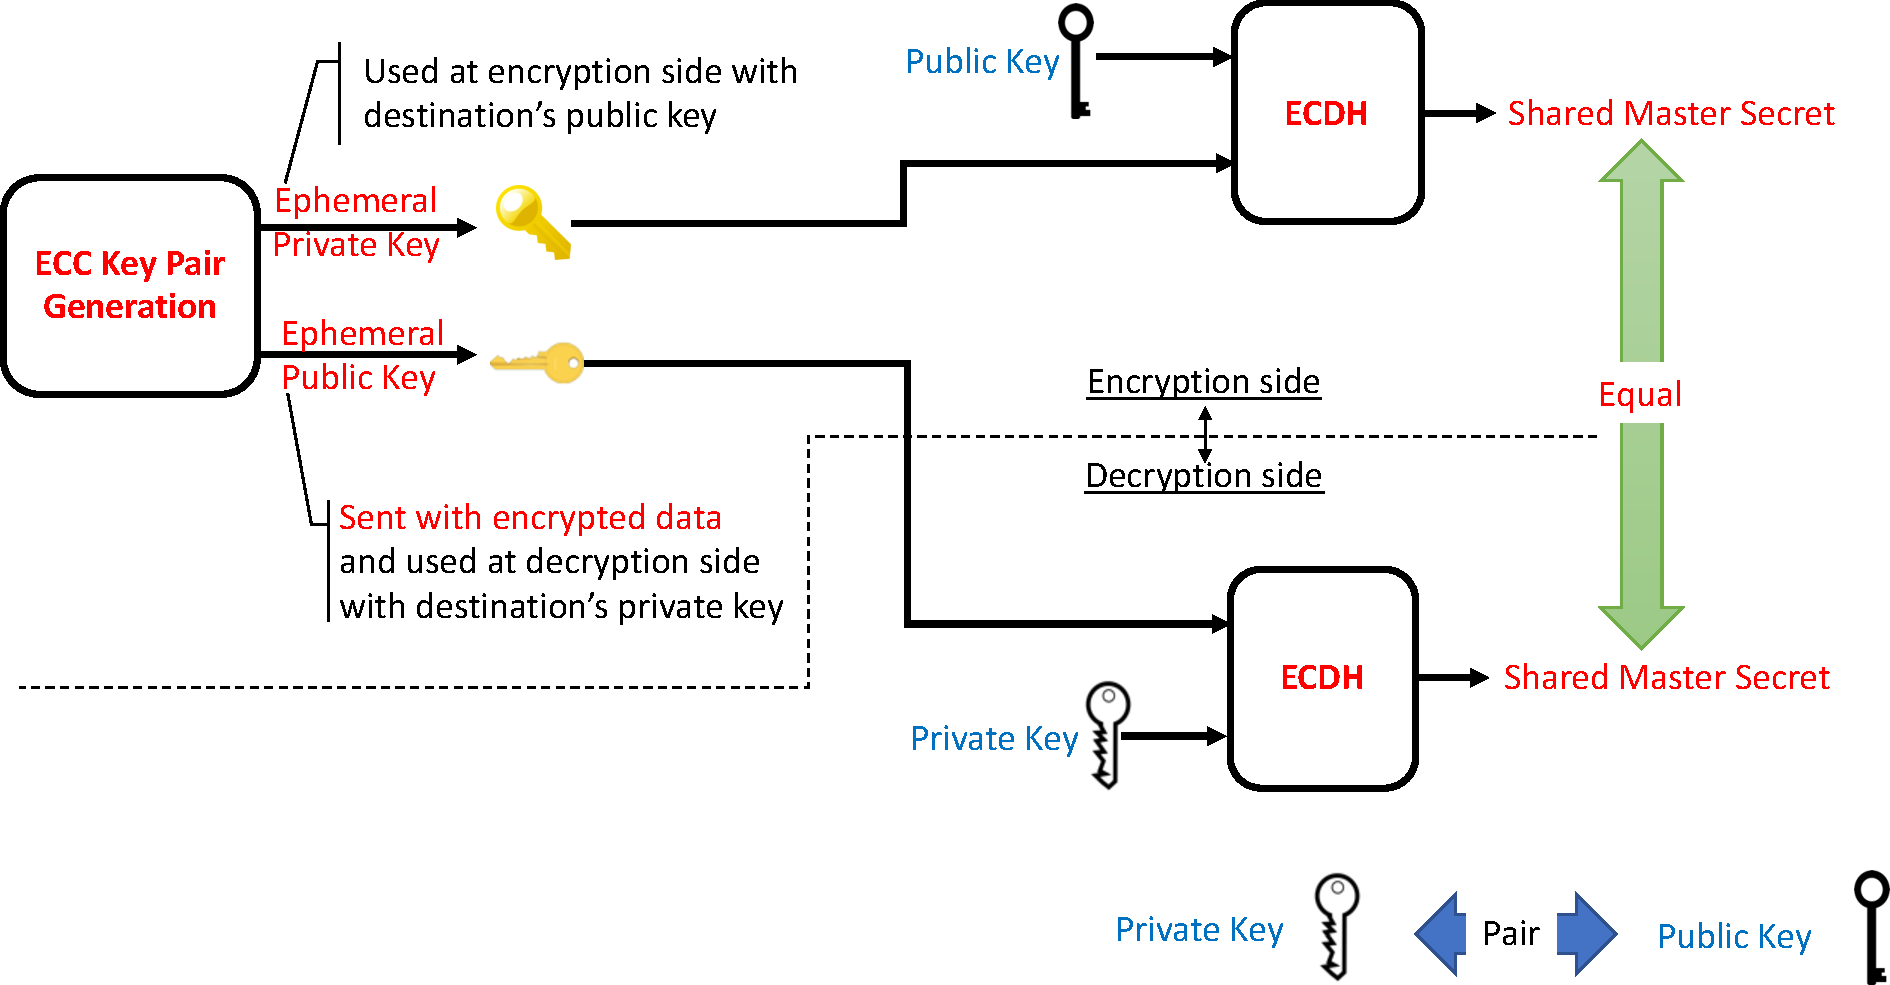
\includegraphics[width=\linewidth]{Figs/ecdh01.pdf}
% \end{center}
% \end{frame}

% \begin{frame}
% \begin{center}
% 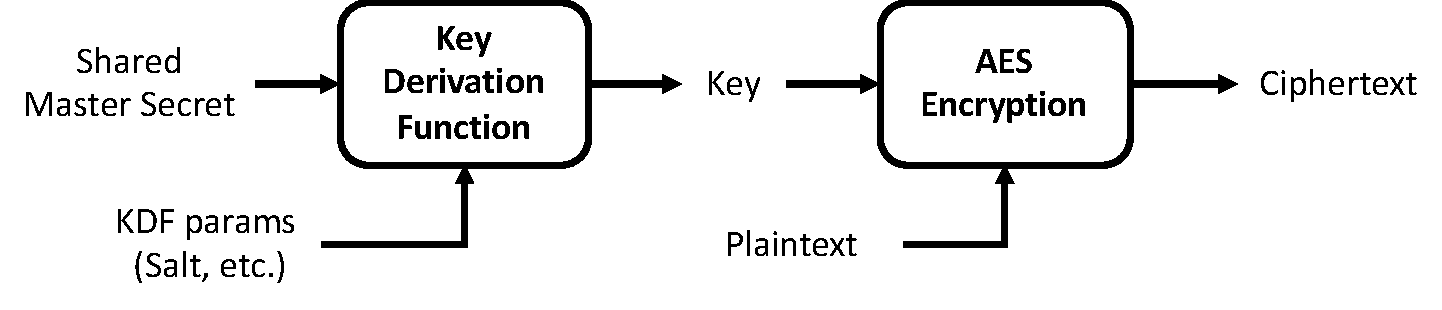
\includegraphics[width=\linewidth]{Figs/ecdh02.pdf}
% \end{center}
% \end{frame}


% \begin{frame}
% \begin{center}
% 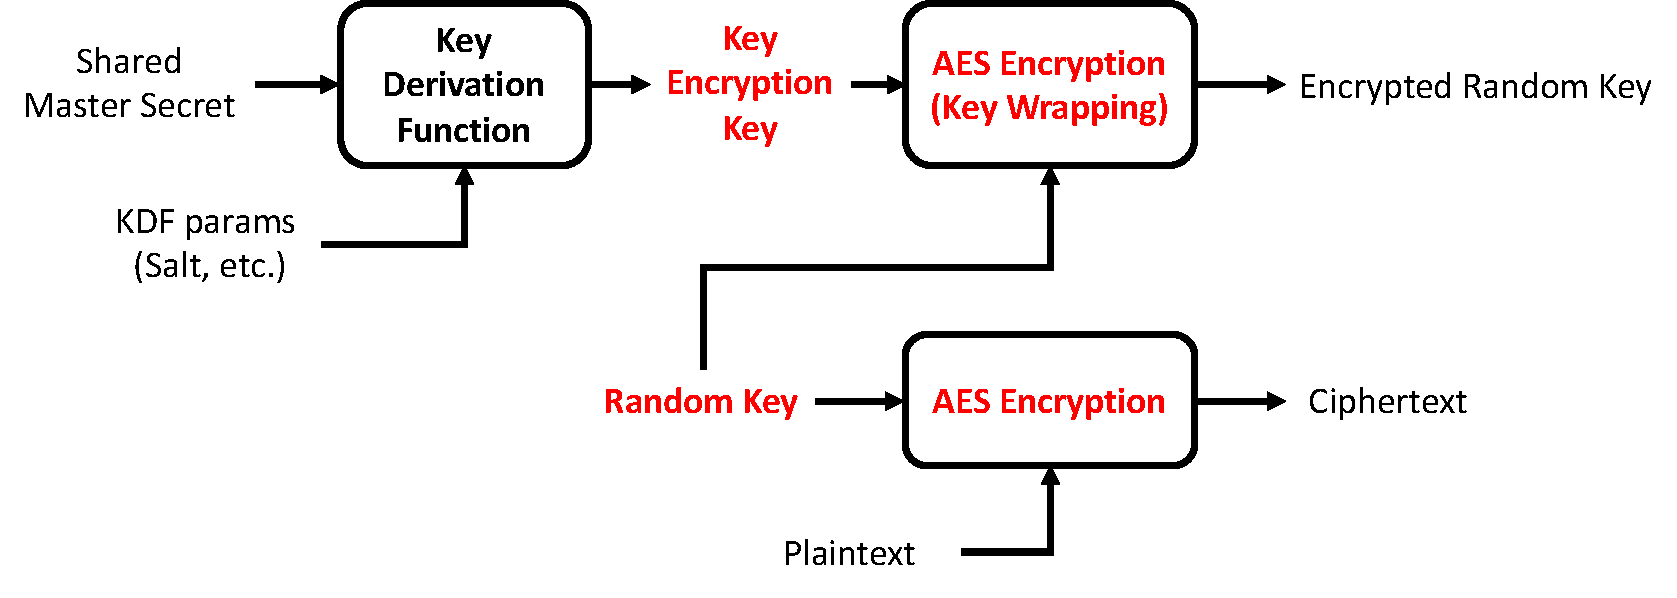
\includegraphics[width=\linewidth]{Figs/aeskw.pdf}
% \end{center}
% \end{frame}




% \section{Backup}

% \begin{frame}
 
% \end{frame}

% \begin{frame}
% \frametitle{Appendix}
% This page is not counted.
% \end{frame}
% \backupend
\end{document}
%%%%%%%%%%%%%%%%%%%%%%%%%%%%%%%%%%%%%%%%%%%%%%%%%%%%%%%%%%%%%%%%%%%%%%%%%%%%%%%%%%%%%%%%%%%%%%%%%%%
%%%%%%%%%%%%%%%%%%%%%%%%%%%%%%%%%%%%%%%%%%%%%%%%%%%%%%%%%%%%%%%%%%%%%%%%%%%%%%%%%%%%%%%%%%%%%%%%%%%
%%%%%%%%%%%%%%%%%%%%%%%%%%%%%%%%%%%%%%%%%%%%%%%%%%%%%%%%%%%%%%%%%%%%%%%%%%%%%%%%%%%%%%%%%%%%%%%%%%%
%%%%%%%%%%%%%%%%%%%%%%%%%%%%%%%%%%%%%%%%%%%%%%%%%%%%%%%%%%%%%%%%%%%%%%%%%%%%%%%%%%%%%%%%%%%%%%%%%%%
%%%%%%%%%%%%%%%%%%%%%%%%%%%%%%%%%%%%%%%%%%%%%%%%%%%%%%%%%%%%%%%%%%%%%%%%%%%%%%%%%%%%%%%%%%%%%%%%%%%
%%%%%%%%%%%%%%%%%%%%%%%%%%%%%%%%%%%%%%%%%%%%%%%%%%%%%%%%%%%%%%%%%%%%%%%%%%%%%%%%%%%%%%%%%%%%%%%%%%%
